As we are interested in understanding the potential energy savings and RH improvement across continental US, we need the weather data collected from major cities across the continent with resolution smaller than every hour. The ISD-lite dataset made available by NOAA (National Oceanographic Association of America) provides air temperature, relative humidity and geographic location at weather stations across major city centers and airports across continental US. This data is publicly available on NOAA’s ftp server. We downloaded a total of 13,800 files for the monitored weather in 2018 for the purpose of this analysis. Since the climate zones, as we are plotting in Figure~\ref{fg:stations}. 

\begin{figure}[h!]
\centering
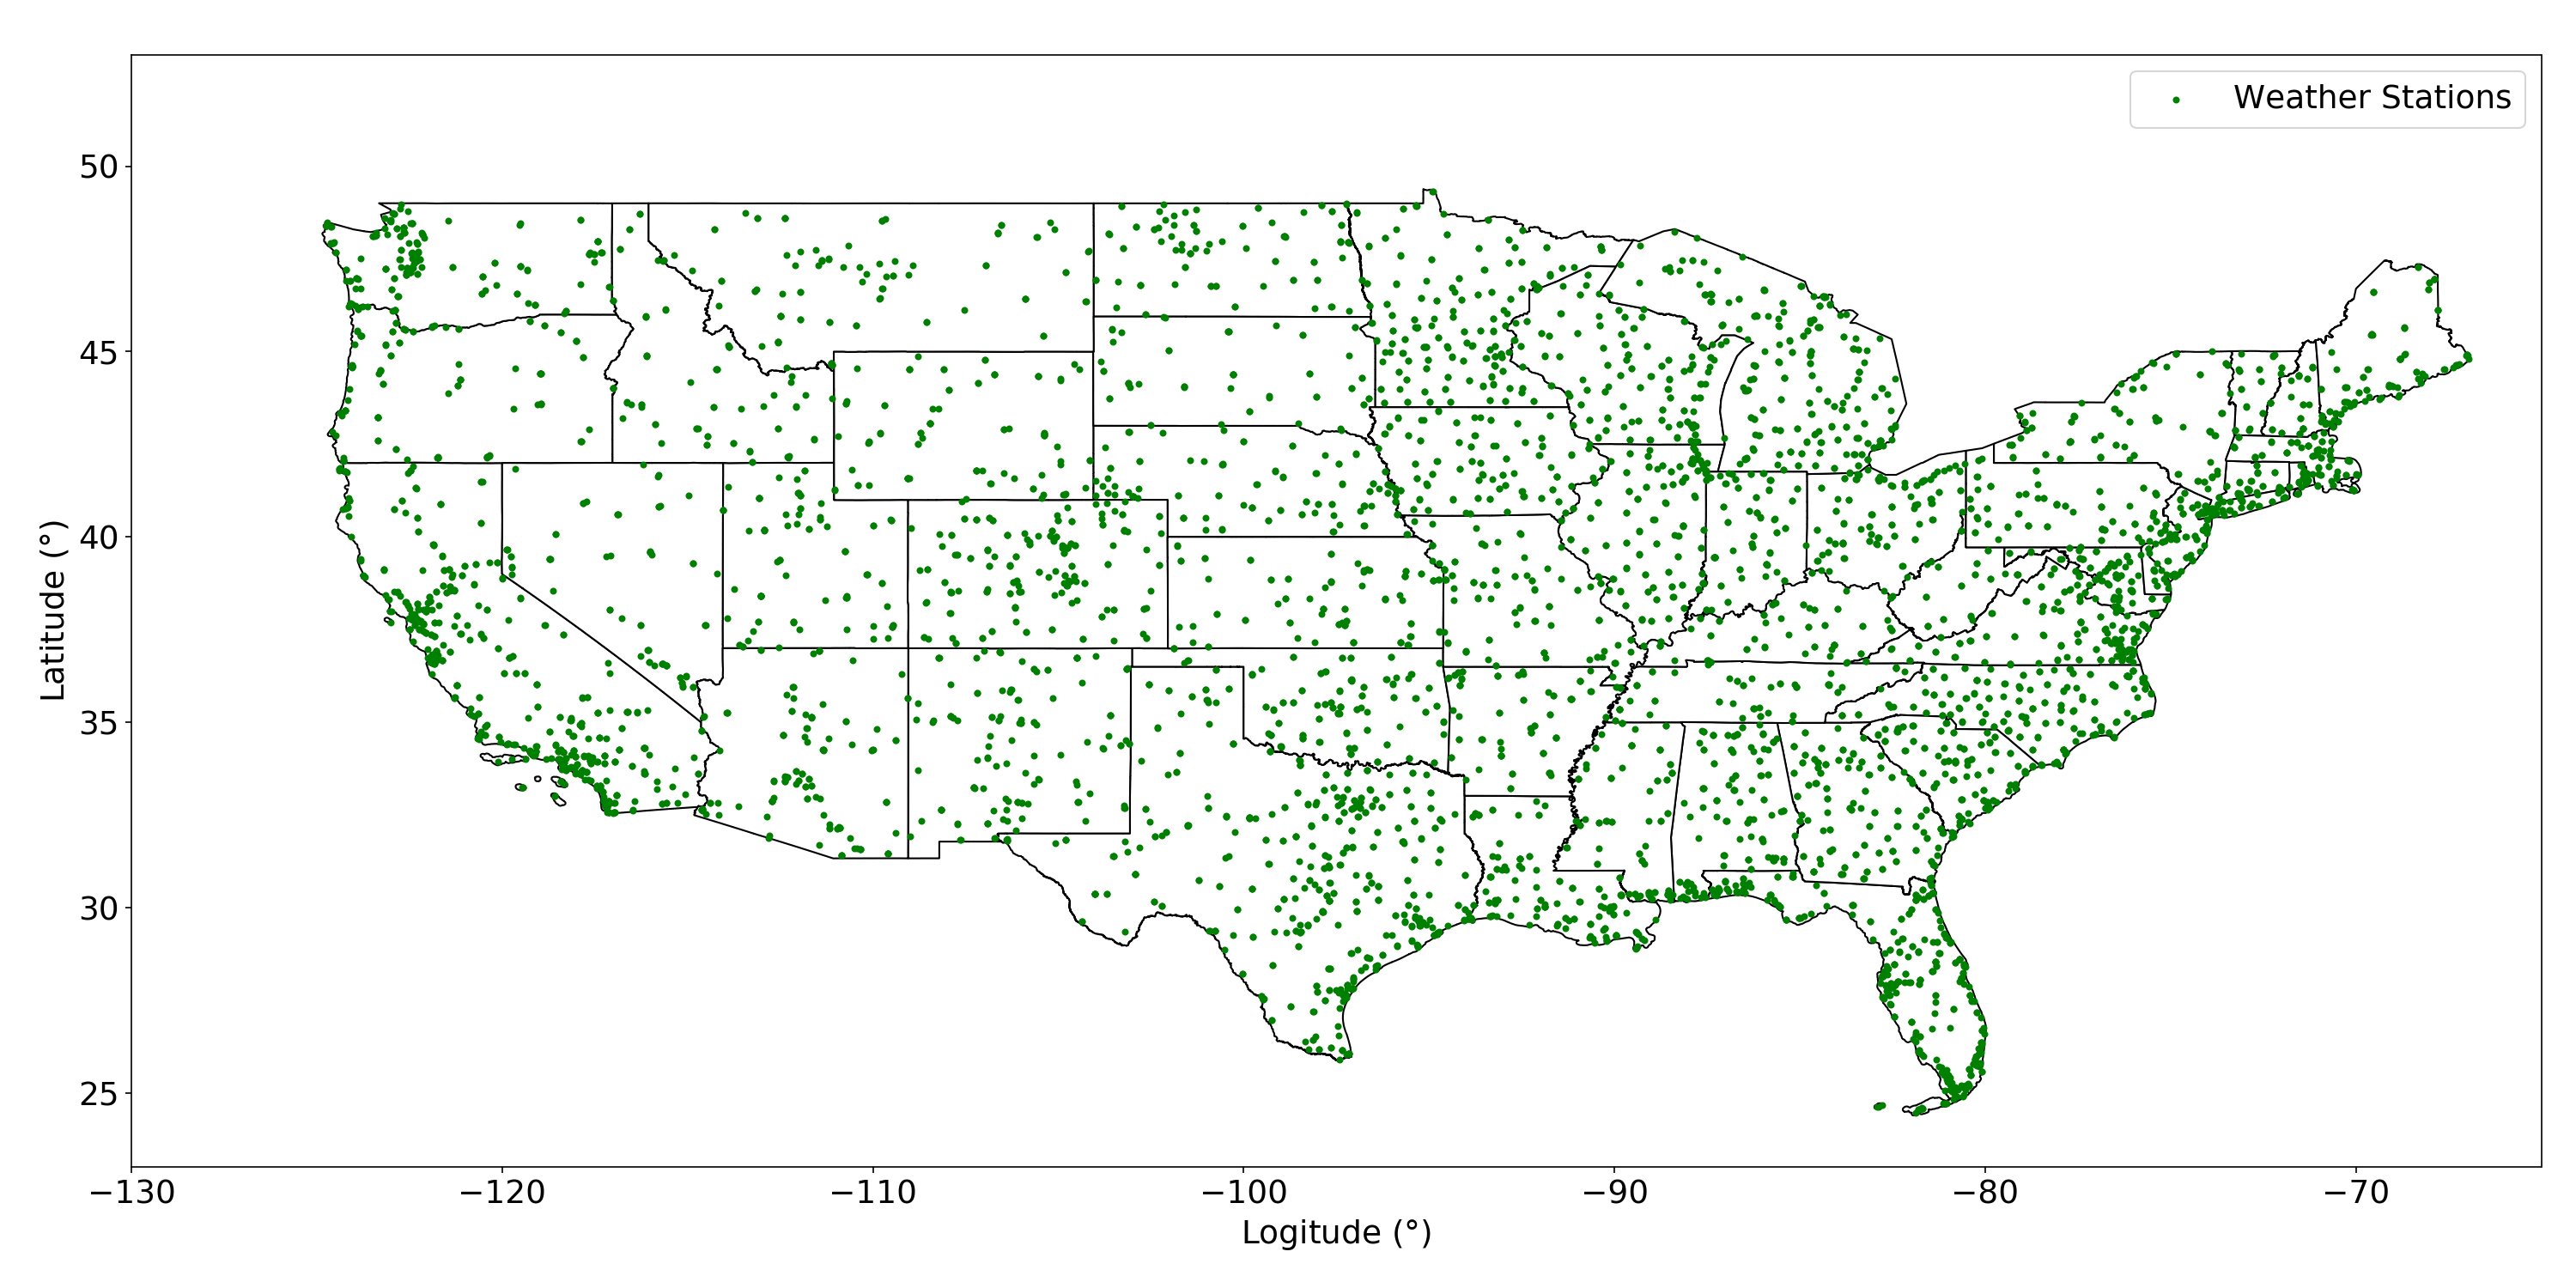
\includegraphics[width=\textwidth]{stations.png}
\caption{Locations of climate station files clipped to the USGS geometry in NOAA ISD-lite, 2017.}\label{fg:stations}
\end{figure}

Upon scraping the NOAA ftp server for the 2018 weather files, we used the pandas data frame library in Python to clean up and regroup the files into time-stamped weather data, and re-sampled on an hourly rate. We also used the CoolProps library to calculate the enthalpy of moist air at different states, and appended the resulting hourly enthalpy states. The resulting weather files will therefore have the air temperature, relative humidity, specific enthalpy for 8760 hours in 2018 across all the stations. We are plotting an example of the data collected in one of the weather stations in Figure~\ref{fg:sampleh}.


\begin{figure}
\centering
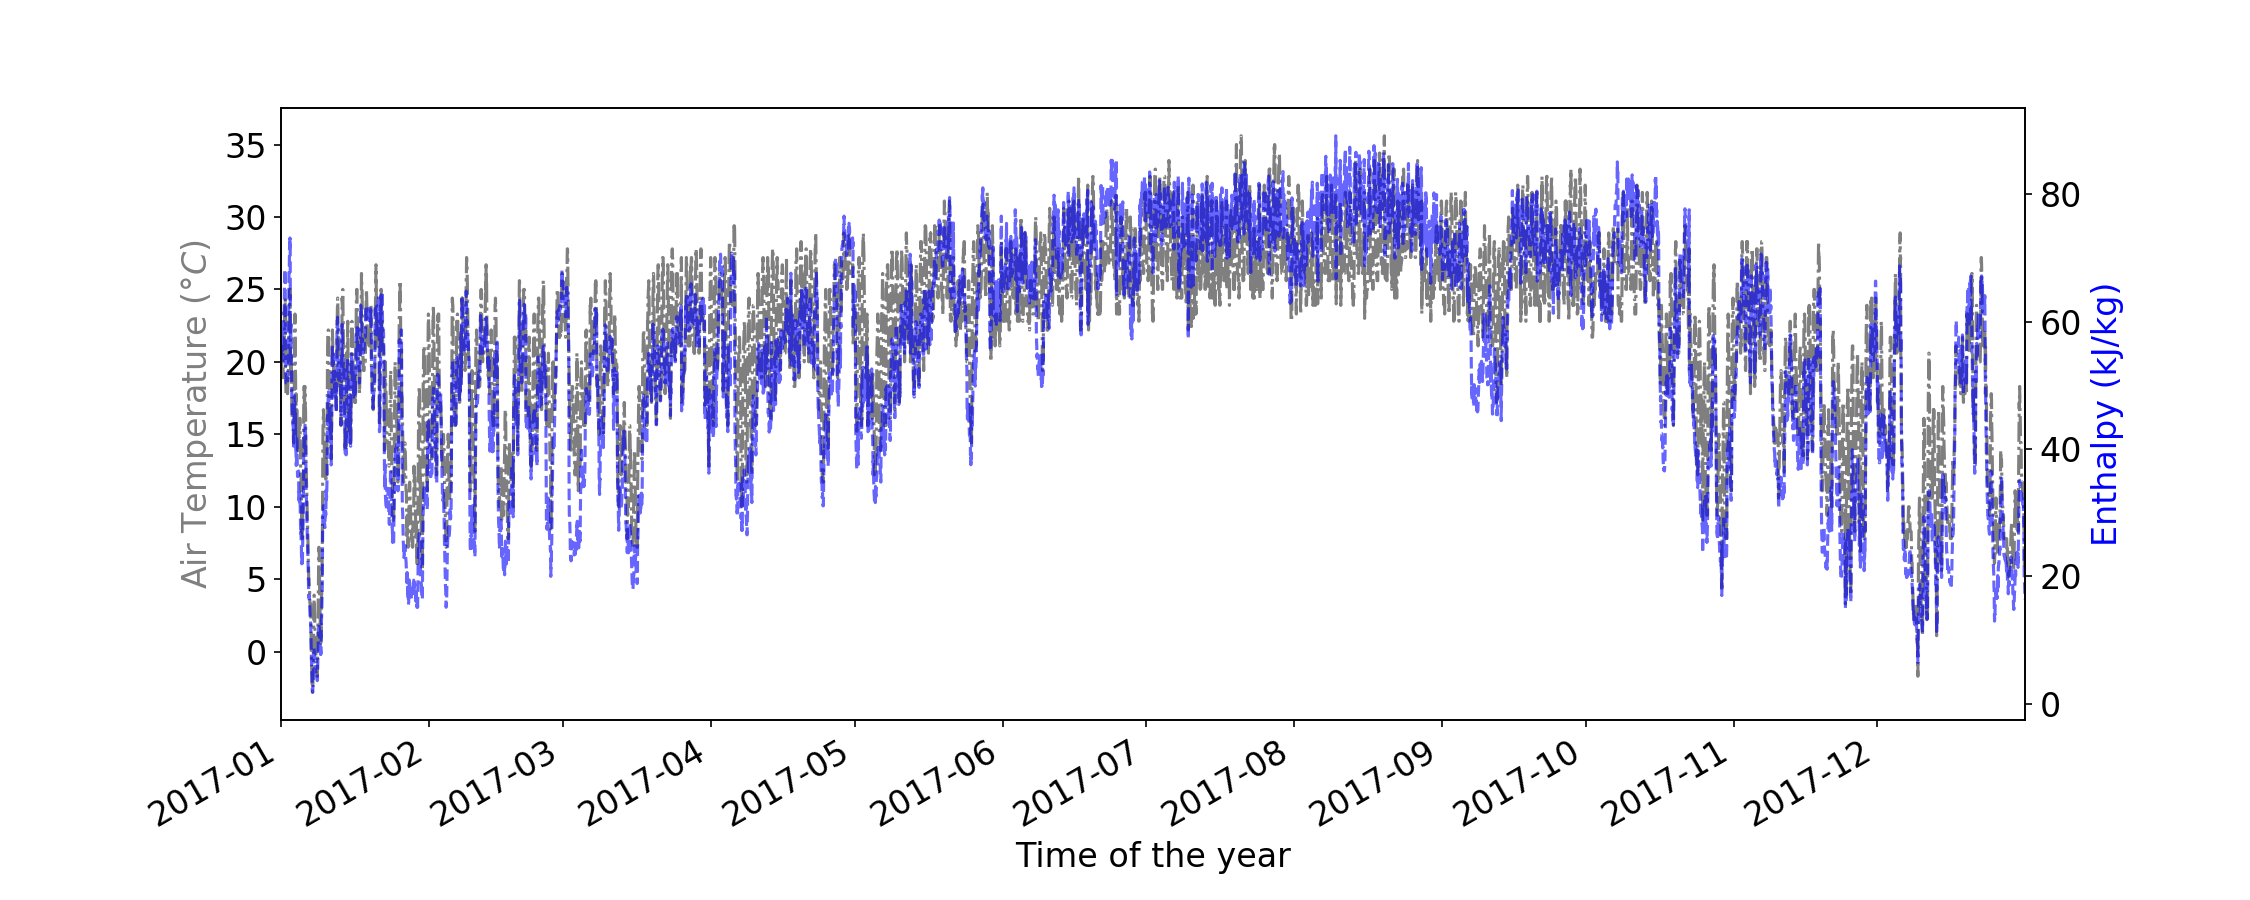
\includegraphics[width=\textwidth]{tbd_h.png}
\caption{ Processed Outdoor Dry-bulb temperature against outdoor specific enthalpy for the weather station in Station ID.}\label{fg:sampleh}
\end{figure}


We will primarily divide our analysis into two parts. The first part focuses on the energy savings of the cooling scenario and the RH improvements for the average heating/cooling condition for the weather stations. 

The second part will examine the entire time series of weather data across different climate zones. 
